\chapter{Lattice Boltzmann}



\section{Expansión de Chapman-Enskog}

\noindent La dinámica macroscópica del fluido se puede ver como el resultado de un comportamiento colectivo de las partículas microscópicas en el sistema de estudio. Naturalmente el formalismo que describe esto de manera adecuada serán las ecuaciones de Navier Stokes\eqref{NS} con las consideraciones de conservación, para poder llegar a las ecuaciones macroscópicas a partir del método de Lattice Boltzmann se utiliza una perturbación del equilibrio. Para empezar a introducir este formalismo de manera más clara, se debe considerar la ecuación de Boltzmann\eqref{Boltzmann} sin dimensión  esto con el fin de entender de mejor manera las escalas en las cuales se posiciona nuestro sistema. Vamos a denotar las cantidades sin dimensión con $\widetilde{x}$ y un número característico apropiado , definimos

\begin{eqnarray}
\widetilde{t} &=& \frac{\xi_{o}}{x_{o}} t \qquad \widetilde{x} = \frac{x}{x_{o}}\qquad \widetilde{\xi}=\frac{\xi}{\xi_{o}}\nonumber\\
\widetilde{\tau} &=& \frac{\xi_{o}}{\overline{x}}\tau\qquad \widetilde{F} = \frac{x_{o}}{\rho\xi_{o}^{2}}F\qquad \widetilde{f} = \frac{c_{o}^{3}}{\rho}f
\end{eqnarray}

\noindent cuando se utilizan las anteriores definiciones sobre la ecuación de Boltzmann se encuentra que en terminos de las variables sin dimensiones se llega a la siguiente ecuación de Boltzmann sin dimensiones

\begin{eqnarray}
\frac{\overline{x}}{x_{o}}\left(\frac{\partial \widetilde{f}}{\partial \widetilde{t}}+\widetilde{\xi}_{\alpha}\frac{\partial \widetilde{f}}{\partial \widetilde{x}_{\alpha}}+\widetilde{F}_{\alpha}\frac{\partial \widetilde{f}}{\partial \widetilde{\xi}_{\alpha}}\right)=-\frac{1}{\widetilde{\tau}}\left(\widetilde{f}-\widetilde{f}^{(0)}\right)
\end{eqnarray}

\noindent entonces se encuentra el numero de Knudsen 

\begin{eqnarray}
\label{Kn}
\text{Kn} = \frac{\overline{x}}{x_{o}}=\frac{\overline{t}}{t_{o}}
\end{eqnarray}

\noindent en donde $\overline{x}$ es el camino libre medio y $\overline{t} = \overline{x}/\xi_{o}$ el tiempo libre medio. Sí $\text{Kn}\rightarrow0$ ambos lados de la ecuación van a cero, el lado izquierdo por la definición del numero de Knudsen, por otro lado, el lado izquierdo se anula porque la función de distribución es muy parecida a la función de equilibrio. Vemos que en cuanto Kn se hace más grande se desvía del equilibrio el sistema, entonces se introduce un pequeño parámetro $\epsilon$ para hacer una expansión y poder perturbar la ecuación de Boltzmann, entonces se introduce

\begin{eqnarray}
f_{i} = \sum_{n=0}^{+\infty}\epsilon^{n}f_{i}^{(n)}\qquad \frac{\partial}{\partial t} = \sum_{n=0}^{+\infty}\epsilon^{n}\frac{\partial}{\partial t_{n}}\qquad\frac{\partial}{\partial x_{\alpha}} = \sum_{n=0}^{+\infty}\epsilon^{n}\frac{\partial}{\partial x_{\alpha}^{n}}\qquad\frac{\partial}{\partial \xi_{\alpha}} = \sum_{n=0}^{+\infty}\epsilon^{n}\frac{\partial}{\partial \xi_{\alpha}^{n}}
\end{eqnarray}

\noindent el primer paso para poder discretizar la ecuación de Boltzmann es poder poner la velocidad en vectores discretos, para esto se utiliza una proyección en la base de hermite de la funcion de distribución de Boltzmann \cite{kruger}. Encontramos que la función de equilibrio discreta tiene la siguiente forma 

\begin{eqnarray}
\label{equilibrio}
\boxed{
f_{i}^{(0)} = \rho w_{i}\left(1+\frac{\xi_{i\alpha}u_{\alpha}}{c_{o}^{2}}+\frac{\xi_{i\alpha}\xi_{i\beta}u_{\alpha}u_{\beta}}{2c_{o}^{4}}-\frac{u_{\alpha}u_{\alpha}}{2c_{o}^{2}}\right)
}
\end{eqnarray}

\noindent en este caso consideramos la parte clásica de los fluidos, porque consideramos la ecuación discreta sin termino de forzamiento, entonces estamos trabajando sobre un formalismo para poder simular las ecuaciones de Navier Stokes 

\begin{eqnarray}
\label{latticeFluidos}
\boxed{\frac{\partial f_{i}}{\partial t}+\xi_{i\alpha}\frac{\partial f_{i}}{\partial x_{\alpha}}=-\frac{1}{\tau}\left(f_{i}-f_{i}^{(0)}\right)}
\end{eqnarray}

Ahora para poder tener la parte discreta de la anterior ecuación se usa el teorema fundamental del cálculo, obteniendo 

\begin{eqnarray}
f_{i}(\vec{x}+\vec{\xi}\Delta t, t + \Delta t)&-&f_{i}(\vec{x},t) \nonumber\\
&=&- \frac{1}{\tau}\int_{0}^{\Delta t}[f_{i}(\vec{x}+\vec{\xi}\lambda, t + \lambda)-f_{i}^{(0)}(\vec{x}+\vec{\xi}\lambda, t + \lambda)]d\lambda
\end{eqnarray}

\noindent para los cálculos utilizados en estos estudios se utiliza el primer orden de discretización entonces se utiliza la siguiente ecuación 


\begin{eqnarray}
\label{LBdiscreta}
f_{i}(\vec{x}+\vec{\xi}\Delta t, t + \Delta t)-f_{i}(\vec{x},t)  
=- \frac{1}{\tau}[f_{i}(\vec{x}, t)-f_{i}^{(0)}(\vec{x}, t)]
\end{eqnarray}


El resultado es explícito en el tiempo, el valor de la función de distribución en el siguiente paso depende del paso actual



\section{Fluidos}

Cuando se considera la ecuación discreta \eqref{latticeFluidos} se debe escoger un conjunto de velocidades discretas adecuadas para poder solucionar tal ecuación, a partir de la definición de los momentos \eqref{momentos} macroscópicos podemos plantear expresiones que permitan calcular las características del fluidos cuando estamos en el sistema discreto, por ejemplo 

\begin{eqnarray}
\label{densidad}
\sum_{i}f_{i}^{(0)}(\vec{x},t) &=& \rho(\vec{x},t)\\
\label{momento}
\sum_{i}\xi_{i\alpha}f_{i}^{(0)}(\vec{x},t) &=& \rho(\vec{x},t)u_{\alpha}(\vec{x},t)\\
\label{momento2}
\sum_{i}\xi_{i\alpha}\xi_{i\beta}f_{i}^{(0)}(\vec{x},t) &=& \Pi_{\alpha\beta}^{(0)}(\vec{x},t)\\
\label{momento3}
\sum_{i}\xi_{i\alpha}\xi_{i\beta}\xi_{i\gamma}f_{i}^{(0)}(\vec{x},t) &=& \Pi_{\alpha\beta\gamma}^{(0)}(\vec{x},t)
\end{eqnarray}

\noindent estas definiciones nos ayudan a imponer condiciones sobre la velocidad discreta, que hace que el sistema físico cobre sentido, vamos a utilizar las anteriores ecuaciones para deducir tales condiciones y la función de equilibrio propuesta \eqref{equilibrio}, lo primero será utilizar la densidad, en este caso 

\begin{eqnarray}
\rho &=& \sum_{i}f_{i}^{0}\nonumber\\
&=&\rho\left[\sum_{i}w_{i}+\frac{u_{\alpha}}{c_{o}^{2}}\sum_{i}w_{i}\xi_{i\alpha}+\frac{u_{\alpha}u_{\beta}}{2c_{o}^{4}}\sum_{i}w_{i}\xi_{i\alpha}\xi_{i\beta}-\frac{u_{\alpha}u_{\alpha}}{2c_{o}^{2}}\sum_{i}w_{i}\right]
\end{eqnarray}


\noindent para que las expresiones sean iguales el termino entre paréntesis cuadrados debe ser cero, entonces resultan las siguientes condiciones 

\begin{eqnarray}
\label{condicion1}
\sum_{i}w_{i}=1\qquad \sum_{i}w_{i}\xi_{i\alpha} = 0 \qquad \sum_{i}w_{i}\xi_{i\alpha}\xi_{i\beta}=c_{o}^{2}\delta_{\alpha\beta}
\end{eqnarray}

\noindent son las tres primeras condiciones para las velocidades y pesos utilizando el momento cero . Ahora se utiliza el primer momento, entonces se tiene

\begin{eqnarray}
\rho u_{\alpha} &=& \sum_{i}\xi_{i\alpha}f_{i}^{(0)}\nonumber\\
&=&\rho\left[\cancelto{0}{\sum_{i}w_{i}\xi_{i\alpha}}+\frac{u_{\alpha}}{c_{o}^{2}}\sum_{i}w_{i}\xi_{i\alpha}\xi_{i\beta}+\frac{u_{\alpha}u_{\beta}}{2c_{o}^{2}}\sum_{i}w_{i}\xi_{i\alpha}\xi_{i\beta}\xi_{i\gamma}-\frac{u_{\alpha}u_{\alpha}}{2c_{o}^{2}}\cancelto{0}{\sum_{i}w_{i}xi_{i\alpha}}\quad\right]\nonumber\\
&=&\rho\underbrace{\left[\frac{u_{\alpha}}{c_{o}^{2}}\sum_{i}w_{i}\xi_{i\alpha}\xi_{i\beta}+\frac{u_{\alpha}u_{\beta}}{2c_{o}^{2}}\sum_{i}w_{i}\xi_{i\alpha}\xi_{i\beta}\xi_{i\gamma}\right]}_{u_{\alpha}}
\end{eqnarray}

Utilizando la última ecuación de \eqref{condicion1} se hace necesario imponer la siguiente condición para poder obtener el momento macroscópico

\begin{eqnarray}
\label{condicion2}
\sum_{i}w_{i}\xi_{i\alpha}\xi_{i\beta}\xi_{i\gamma} = 0 
\end{eqnarray}

\noindent por último se utiliza la condición del segundo momento para evidenciar la última condición que consideramos 

\begin{eqnarray}
\Pi_{\alpha\beta}^{0}&=&\rho u_{\alpha}u_{\beta}+\rho c_{o}^{2}\delta_{\alpha\beta}=\sum_{i}\xi_{i\alpha}\xi_{i\beta}f_{i}^{(0)}\nonumber\\
&=&\rho\left[\sum_{i}w_{i}\xi_{i\alpha}\xi_{i\beta} + \frac{u_{\gamma}}{c_{o}^{2}}\cancelto{0}{\sum_{i}w_{i}\xi_{i\alpha}\xi_{i\beta}}\xi_{i\gamma}+\frac{u_{\gamma}u_{\phi}}{2c_{o}^{4}}\sum_{i}w_{i}\xi_{i\alpha}\xi_{i\beta}\xi_{i\gamma}\xi_{i\phi}-\frac{u_{\gamma}u_{\gamma}}{2c_{o}^{2}}\sum_{i}w_{i}\xi_{i\alpha}\xi_{i\beta}\right]\nonumber\\
&=&\rho c_{o}^{2}\delta_{\alpha\beta}\underbrace{+\frac{u_{\gamma}u_{\phi}}{2c_{o}^{4}}\sum_{i}w_{i}\xi_{i\alpha}\xi_{i\beta}\xi_{i\gamma}\xi_{i\phi}-\frac{u_{\gamma}u_{\gamma}}{2}\delta_{\alpha\beta}}_{=\rho u_{\alpha}u_{\beta}}
\end{eqnarray}

\noindent utilizando la ayuda de la delta de kronecker se puede exigir la condición del momento de la siguiente manera, completando las condiciones sobre las velocidades y los pesos

\begin{eqnarray}
\sum_{i}w_{i}\xi_{i\alpha}\xi_{i\beta}\xi_{i\gamma}\xi_{i\phi} = c_{o}^{4}(\delta_{\alpha\beta}\delta_{\gamma\phi}+\delta_{\alpha\gamma}\delta_{\beta\phi}+\delta_{\alpha\phi}\delta_{\beta\gamma})
\end{eqnarray}

\noindent hasta el momento se tienen las condiciones para poder encontrar el conjunto de velocidades que respete las definiciones macroscópicas. Ahora para poder tener la parte discreta de la ecuacion de Boltzmann \eqref{LBdiscreta} se hace una expansión en serie de Fourier de la ecuación de evolución del sistema 

\begin{eqnarray}
\label{expansion}
f_{i}(\vec{x}+\vec{\xi_{i}}\Delta t, t + \Delta t)-f_{i}(\vec{x},t) = \Delta t \frac{\partial f_{i}}{\partial x_{\alpha}}\xi_{i\alpha} &+& \Delta t \frac{\partial f_{i}}{\partial t} + \frac{\Delta t^{2}}{2}\frac{\partial^{2}f_{i}}{\partial x_{\alpha} \partial x_{\beta}}\xi_{i\alpha}\xi_{i\beta}+\nonumber\\\frac{\Delta t^{2}}{2}\frac{\partial^{2}f_{i}}{\partial t^{2}}
&+& \Delta t^{2} \frac{\partial^{2}f_{i}}{\partial x_{\alpha}\partial t}\xi_{i\alpha} = -\frac{1}{\tau}(f_{i}-f^{eq}_{i})
\end{eqnarray}

\noindent en donde los índices griegos denotan la dimensión del sistema en estudio. Para reproducir las ecuaciones de Navier-Stokes se aplica una expansión de Chapman-Enskog usando un parámetro $\epsilon$


\begin{eqnarray}
f_{i} = \sum_{n=0}^{\infty} \epsilon^{n} f_{i}^{(n)}, \qquad \frac{\partial}{\partial t} = \sum_{n = 0}^{\infty}\epsilon^{n}\frac{\partial}{\partial t_{n}}
\end{eqnarray}

\noindent Tomando el número de Knudsen\eqref{Kn} se puede identificar que el parámetro perturvativo $\epsilon = \Delta t$ en la ecuación de Boltzmann discretizada\eqref{LBdiscreta} \cite{principal} en donde, ahora reemplazando en la expansión de Taylor \eqref{expansion}  las definiciones de los términos perturvativos se tiene que 

\begin{eqnarray}
&\Delta t&\left(\xi_{i\alpha}\frac{\partial}{\partial x_{\alpha}}\left(f_{i}^{(0)}+\epsilon f_{i}^{(1)} + \epsilon^{2} f_{i}^{(2)}\right) + \left(\frac{\partial}{\partial t_{0}} + \epsilon \frac{\partial}{\partial t_{1}} \right)\left(f_{i}^{(0)}+\epsilon f_{i}^{(1)} + \epsilon^{2} f_{i}^{(2)}\right)\right)\nonumber \\
&+&\frac{\Delta t^{2}}{2}\left(\xi_{i\alpha}\xi_{i\beta}\frac{\partial^{2}}{\partial x_{\alpha}\partial x_{\beta}}\left(f_{i}^{(0)}+\epsilon f_{i}^{(1)} + \epsilon^{2} f_{i}^{(2)}\right)+\left(\frac{\partial}{\partial t_{0}} + \epsilon \frac{\partial}{\partial t_{1}} \right)^{2}\left(f_{i}^{(0)}+\epsilon f_{i}^{(1)} + \epsilon^{2} f_{i}^{(2)}\right)\right)\nonumber \\
&+&\frac{\Delta t^{2}}{2}\left(\xi_{i\alpha}\left(\frac{\partial}{\partial x_{\alpha}}\right)\left(\frac{\partial}{\partial t_{0}} + \epsilon \frac{\partial}{\partial t_{1}} \right)\left(f_{i}^{(0)}+\epsilon f_{i}^{(1)} + \epsilon^{2} f_{i}^{(2)}\right)\right) \nonumber\\
&=& -\frac{1}{\tau}\left(\left(f_{i}^{(0)}+\epsilon f_{i}^{(1)} + \epsilon^{2} f_{i}^{(2)}\right)-f_{i}^{eq}\right)
\end{eqnarray}

\noindent si se compara los términos de orden cero, uno y dos se pueden encontrar las siguientes relaciones 

\begin{eqnarray}
\label{momento0}
f_{i}^{0} &=& f_{i}^{eq} \\
\label{momento1}
\frac{\partial f_{i}^{(0)}}{\partial t_{0}} &+& \xi_{i\alpha}\frac{\partial f_{i}^{(0)}}{\partial x_{\alpha}} = -\frac{f_{i}^{(1)}}{\tau} \\
\xi_{i\alpha}\frac{\partial f_{i}^{(1)}}{\partial x_{\alpha}} + \frac{\partial f_{i}^{(1)}}{\partial t_{0}} &+& \frac{\xi_{i\alpha}\xi_{i\beta}}{2}\frac{\partial^{2}f_{i}^{(0)}}{\partial x_{\alpha}\partial x_{\beta}}+\frac{1}{2}\frac{\partial^{2}f_{i}^{(0)}}{\partial t_{0}^{2}}+\nonumber \\
\xi_{i\alpha}\frac{\partial^{2}f_{i}^{(0)}}{\partial t_{0}^{2}}&+&\xi_{i\alpha}\frac{\partial^{2}f_{i}^{(0)}}{\partial x_{\alpha}\partial t_{0}}+\frac{\partial f_{i}^{(0)}}{\partial t_{1}} = -\frac{f_{i}^{(2)}}{\tau} 
\end{eqnarray}

\noindent a partir de \eqref{momento0} y las siguientes sustituciones considerando \eqref{momento1}

\begin{eqnarray}
\xi_{i\alpha}\frac{\partial f_{i}^{(0)}}{\partial x_{\alpha}} = -\frac{f_{i}^{(1)}}{\tau}-\frac{\partial f_{i}^{(0)}}{\partial t_{0}}, \qquad \frac{\partial^{2} f_{i}^{(0)}}{\partial t_{0}^{2}}=-\frac{1}{\tau}\frac{\partial f_{i}^{(1)}}{\partial t_{0}}-\xi_{i\alpha}\frac{\partial^{2}f_{i}^{(0)}}{\partial x_{\alpha}\partial t_{0}}
\end{eqnarray}

\noindent se llega a las ecuaciones que dependen de la función de equilibrio 

\begin{eqnarray}
f_{i}^{eq}=-\frac{f_{i}^{(0)}}{\tau}\\
\frac{\partial f_{i}^{eq}}{\partial t_{0}} + \xi_{i\alpha}\frac{\partial f_{i}^{eq}}{\partial x_{\alpha}} = -\frac{f_{i}^{(1)}}{\tau} \\
\frac{\partial f_{i}^{eq}}{\partial t_{1}}+\left(1-\frac{1}{2\tau}\right)\left(\frac{\partial}{\partial t_{0}}+\xi{i\alpha}\frac{\partial}{\partial x_{\alpha}}\right)f_{i}^{(1)} &=& -\frac{f_{i}^{(2)}}{\tau}.
\end{eqnarray}

\noindent ahora se tiene que las ecuaciones de evolución dependen exclusivamente de la función de equilibrio y de como se quiera hacer propagar la información. 

\noindent Hasta el momento se ha dado el fundamento teórico del método de lattice Boltzmann, consiguiento derivar la ecuación de evlución temporal. Entonces ahora se hace un pequeño resumen, al estilo de receta para la implementación efectiva del método.
\\
\noindent En todos los desarrollo y ejemplos llevados a cabo en el presente trabajo se considera mallas regulares, en donde cada nodo de dicho arreglo contiene $i$ funciones de distribución , en donde $i$ es el número de direcciones de la velocidad discreta. Tal función de distribución representa las partículas con velocidad $\vec{\xi}_{i}4$ en el nodo $\vec{x}$  en un tiempo $t$. Los vectores de velocidad se eligen de tal manera que el nodo actual se relacione con sus vecions más cercanos, con ayuda de las condiciones \eqref{condicion1}\eqref{condicion2}, las funciones de distribución se utilizan para calcular las cantidades macroscópicas físicas usuales \eqref{densidad},\eqref{momento},\eqref{momento2},\eqref{momento3}. En cada paso de tiempo las partículas de cada nodo colisiona, tal proceso se modela  con la función de distribución de equilibrio \eqref{equilibrio} , esta construida desde los momentos macroscópicos y la una distribución Maxweliana. Los coeficientes $w_{i}$ dependen del conjunto de velocidades discretas que se elijan en un problema particular
\noindent Físicamente podemos entender en cada paso de tiempo el siguiente proceso. En cada nodo las partículas colisionan obedeciendo una función de distribución del paso anterior en un tiempo $\tau$ ,llamado tiempo de relajación, llegando al equilibrio $f_{i}^{(0)}$, este proceso define una nueva distribución de partículas para el siguiente paso la cual se comunica a los nodos vecinos, todo este proceso lo evidencia la ecuación \eqref{LBdiscreta}, entonces en concreto. EL algoritmo empieza calculando la densidad y la velocidad desde la función de distribución de partículas , después de esto con los nuevos valores de la densidad y la velocidad se calcula la función de equilibrio $f_{i}^{(0)}$, utilizando \eqref{LBdiscreta} se calcula la distribución post-colisión que se comunica a los vecinos. 

\section{Ejemplos}

\subsection{Flujo de Poiseuille}

\noindent Este problema considera el movimiento de un fluido a traves de un cilindro, 
En el fluido laminar las trayectorias de las partículas no se cruzan. El fluido se considera como cilindros concéntricos los cuales se deslizan unos sobre otros como tubos de telescópicos. La diferencia de velocidades entre cilindros da cuenta de la viscosidad del fluido. Consideramos Navier - Stokes \eqref{NS}

\begin{eqnarray*}
\rho \left(\frac{\partial}{\partial t} + \vec{v}\cdot \nabla\right)\vec{v} = - \nabla p + \eta\nabla^{2} \vec{v} + \vec{F}
\end{eqnarray*}

\noindent Se considera un sistema bidimensional, de manera que $v = u_{x}\hat{x} + u_{y}\hat{y}$, en donde se asume que la velocidad solo depende de $y$, y es nula en la dirección $x$

\begin{eqnarray*}
\rho\frac{\partial u_{x}}{\partial t}\left(u_{x}\frac{\partial}{\partial x} + u_{y}\frac{\partial}{\partial y}\right)u_{x} &=& -\frac{\partial p}{\partial x} + \eta\left(\frac{\partial^{2}}{\partial x^{2}}+\frac{\partial^{2}}{\partial y^{2}}\right)u_{x}\\
\rho\frac{\partial u_{y}}{\partial t}\left(u_{x}\frac{\partial}{\partial x} + u_{y}\frac{\partial}{\partial y}\right)u_{y} &=& -\frac{\partial p}{\partial y} + \eta\left(\frac{\partial^{2}}{\partial x^{2}}+frac{\partial^{2}}{\partial y^{2}}\right)u_{y}-\rho g
\end{eqnarray*}

\noindent No se considera aceleración en el fluido, se tiene:

\begin{eqnarray*}
0 = -\frac{\partial p}{\partial y} + \eta\frac{\partial^{2}u_{y}}{\partial x^{2}} - \rho g \quad\longrightarrow\quad \eta\frac{\partial^{2}u_{y}}{\partial x^{2}} =  \frac{\partial p}{\partial y} +  \rho g
\end{eqnarray*}

\noindent Solucionando la ecuación diferencial se puede ver que 

\begin{eqnarray*}
u_{y} = \frac{1}{2\eta}\left(\frac{\partial p}{\partial y} + \rho g\right)x^{2} + C_{1}x +C_{2}
\end{eqnarray*}

\noindent Considerando las condiciones de frontera 

\begin{eqnarray*}
u_{y}(x = 0) = 0 \qquad u_{y}(x = d) = 0  
\end{eqnarray*}

\noindent Se obtiene 

\begin{eqnarray*}
u_{y} = \frac{1}{2\eta}\left(\frac{\partial p}{\partial y} + \rho g\right)x(x-d)
\end{eqnarray*}

\noindent Que se puede escribir como 

\begin{eqnarray}
\label{TeoricaPoiseuille}
\boxed{u_{y} = \frac{1}{2\eta}\left(\frac{\partial p}{\partial y} + \rho g\right)\left[\left(x-\frac{d}{2}\right)^{2} - \frac{d^{2}}{4}\right]}
\end{eqnarray}


Ahora se define un conjunto de velocidades que respete las condiciones \eqref{condicion1}\eqref{condicion2}, para este caso se elije un conjunto D2Q9

\begin{figure}[H]
\centering
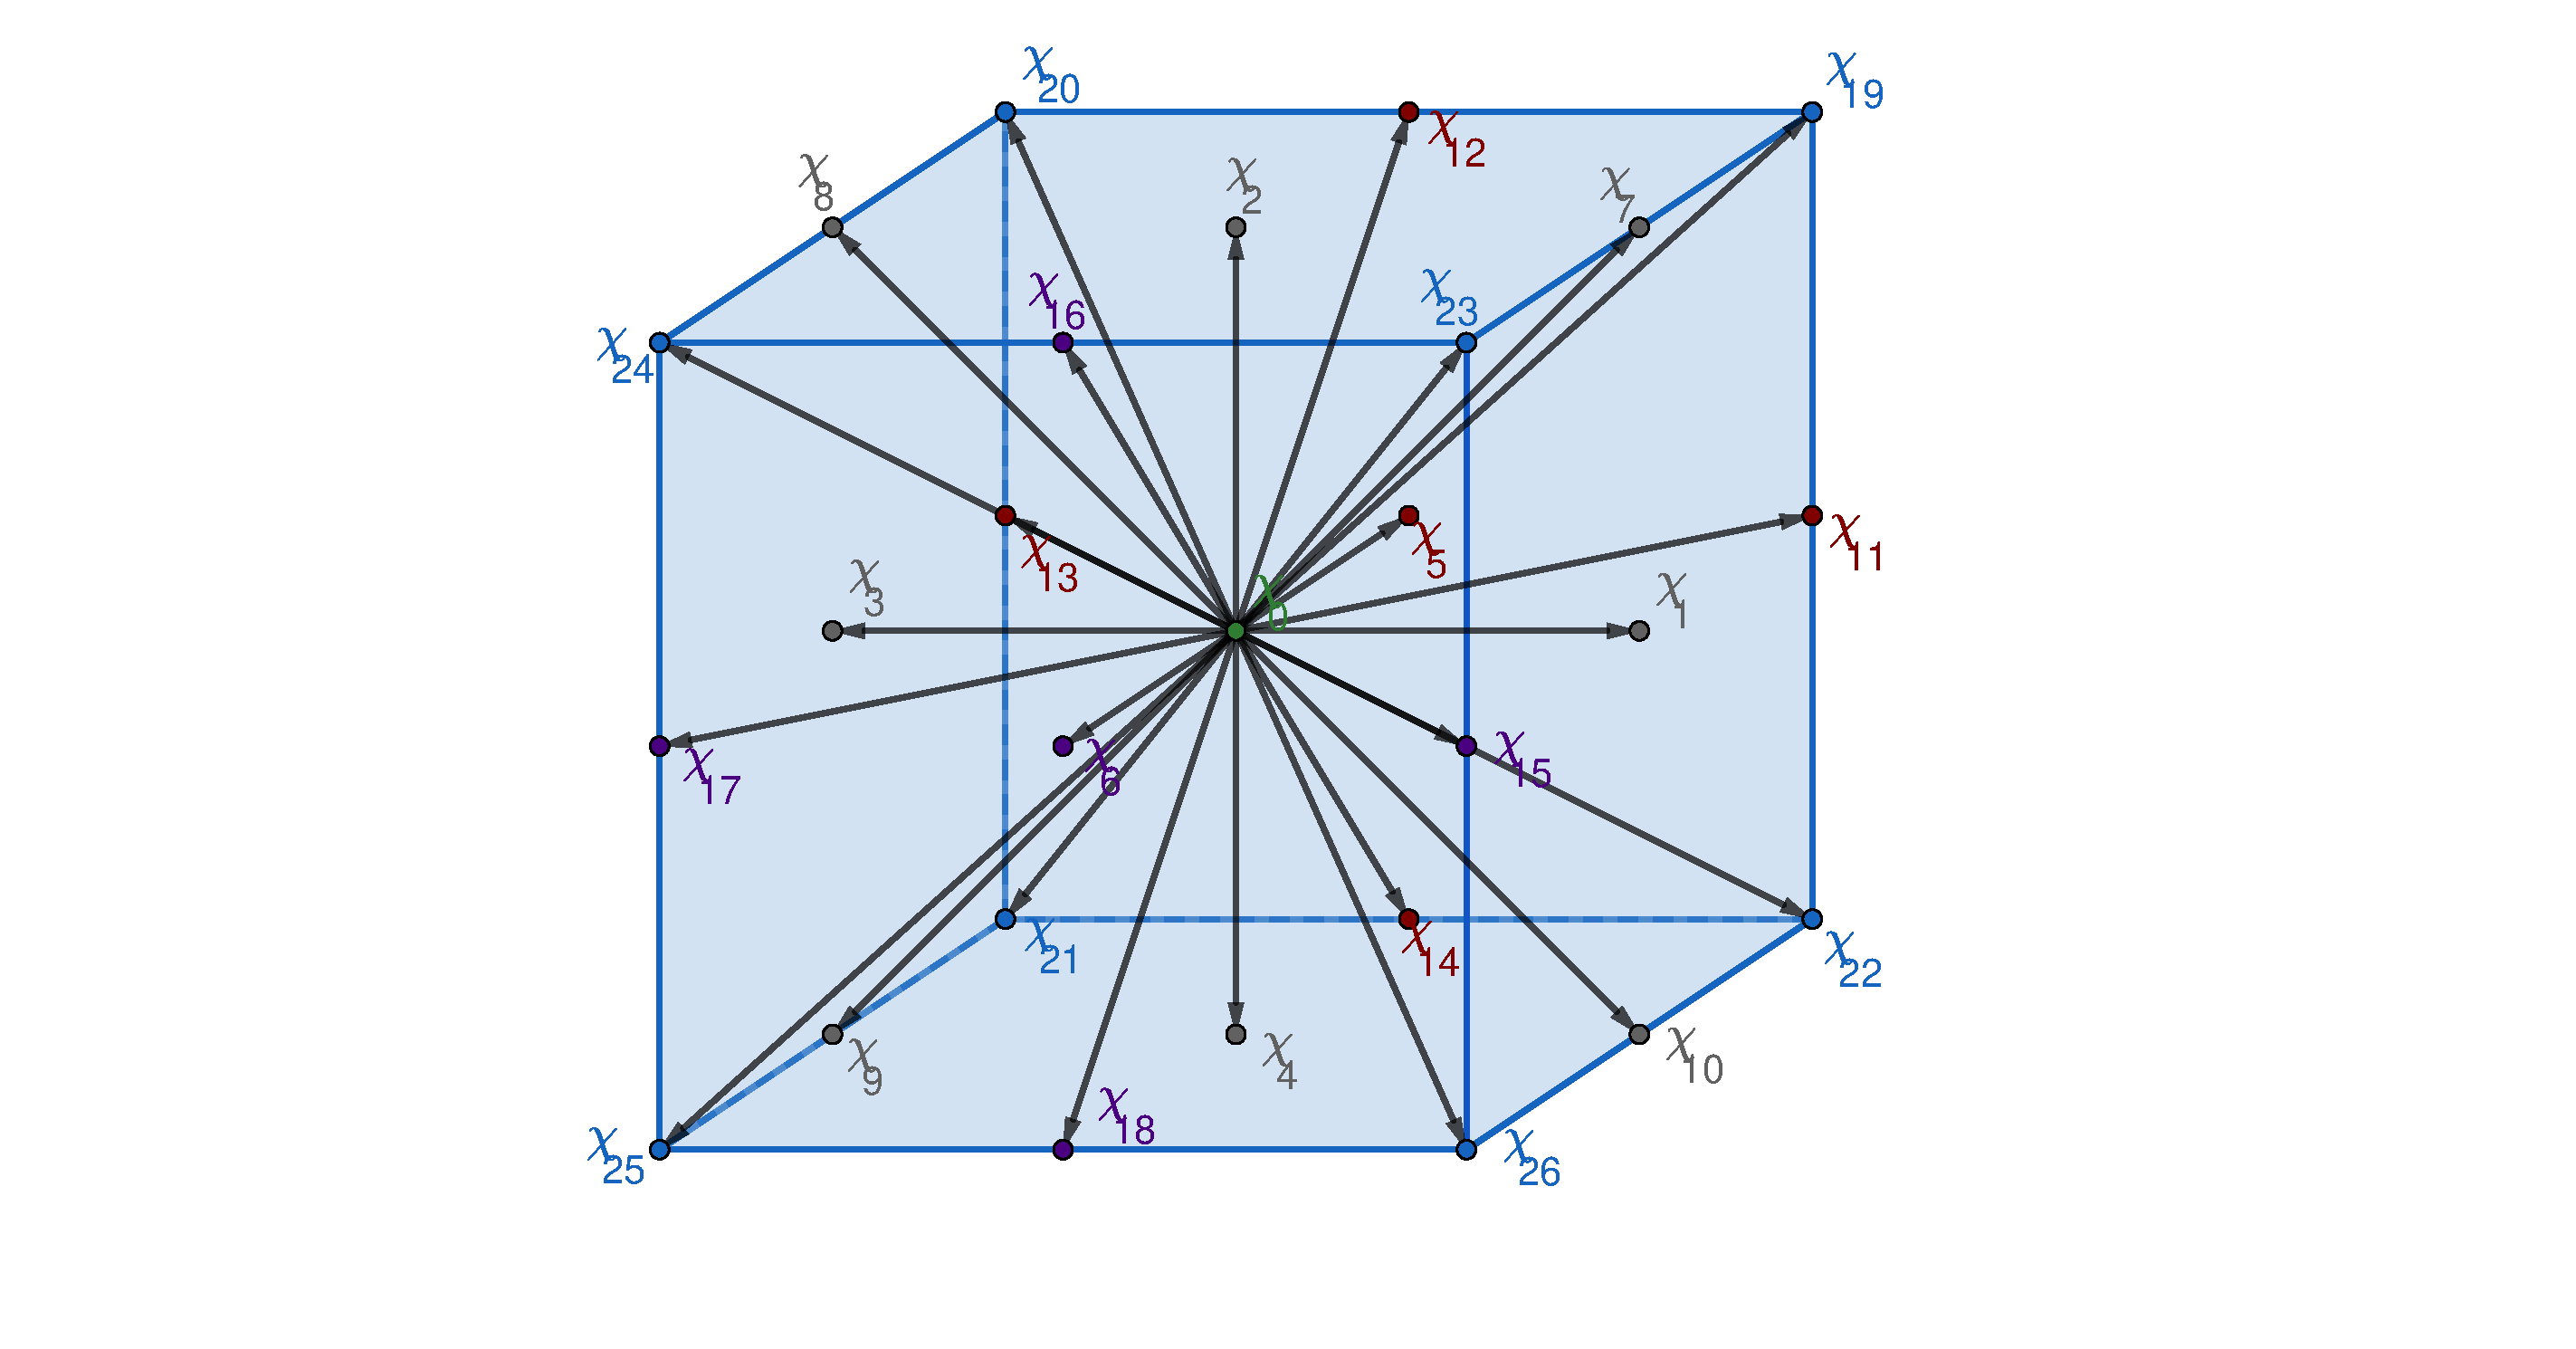
\includegraphics[scale = 0.3]{D3Q19.pdf}
\caption{Elección de los vectores y malla elegida para el sistema bidimensional en el flujo de Poiseuille }
\label{Poiseuille_100}
\end{figure}

la elección mostrada en la anterior figura define $w_{1}=w_{2}=w_{3}=w_{4}=w_{a}$ por otra parte $w_{5}=w_{6}=w_{7}=w_{8}=w_{b}$ obtenemos el siguiente sistema 

\begin{eqnarray}
\sum_{i}w_{i} &=& w_{o}+4w_{a}+4w_{b} = 1\\
\sum_{i}w_{i}\xi^{2}_{i\alpha}&=&\left(\frac{\Delta x}{\Delta t}\right)^{2}(2w_{a}+4w_{b})=c_{o}^{2}\\
\sum_{i}w_{i}\xi_{ix}^{2}\xi_{iy}^{2}&=&\left(\frac{\Delta x}{\Delta t}\right)^{4}4w_{b} = c_{o}^{4}\\
\sum_{i}w_{i}\xi_{i\alpha}^{4} &=& \left(\frac{\Delta x}{\Delta t}\right)^{4}(2w_{a}+4w_{b})=2c_{o}^{4}
\end{eqnarray}

En donde se obtiene

\begin{eqnarray}
c_{o}=\frac{\Delta x}{\Delta t} \frac{1}{\sqrt{3}}, \quad w_{o}=\frac{4}{9}, \quad w_{a} = \frac{1}{9},\quad w_{b}= \frac{1}{36}
\end{eqnarray}


\begin{figure}[H]
\label{perfiles}
\centering
\begin{subfigure}
\centering
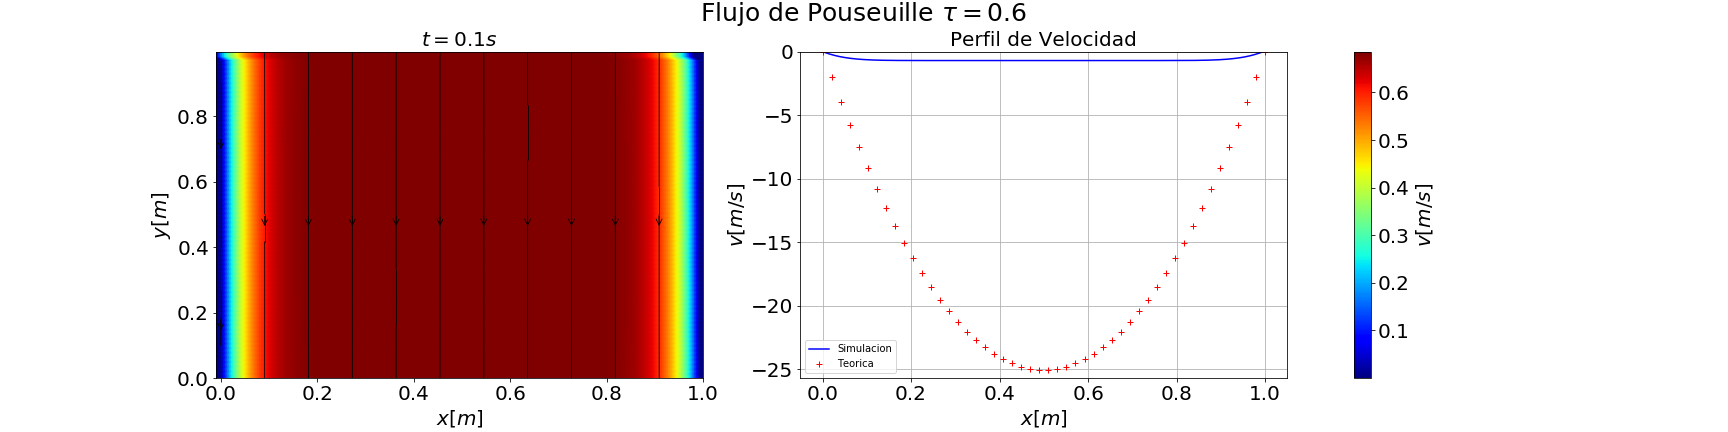
\includegraphics[scale=0.32]{01s.png} 
%\caption{Generic} \label{fig:timing1}
\end{subfigure}

\begin{subfigure}
\centering
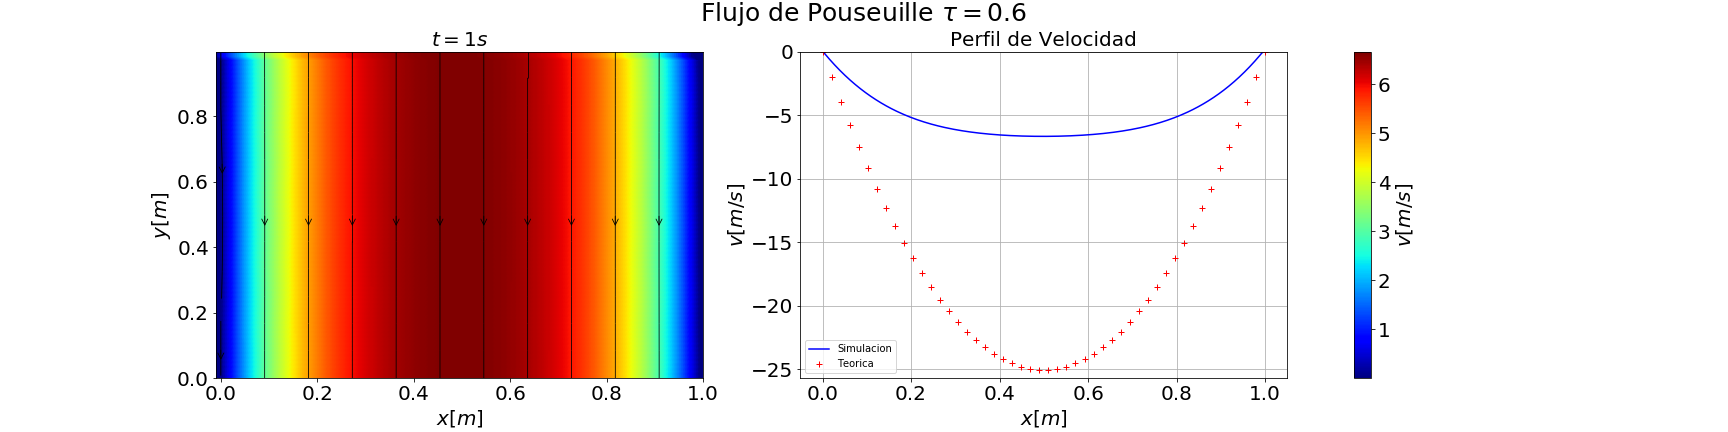
\includegraphics[scale=0.32]{1s.png} 
%\caption{Competitors} \label{fig:timing2}
\end{subfigure}

\begin{subfigure} 
\centering
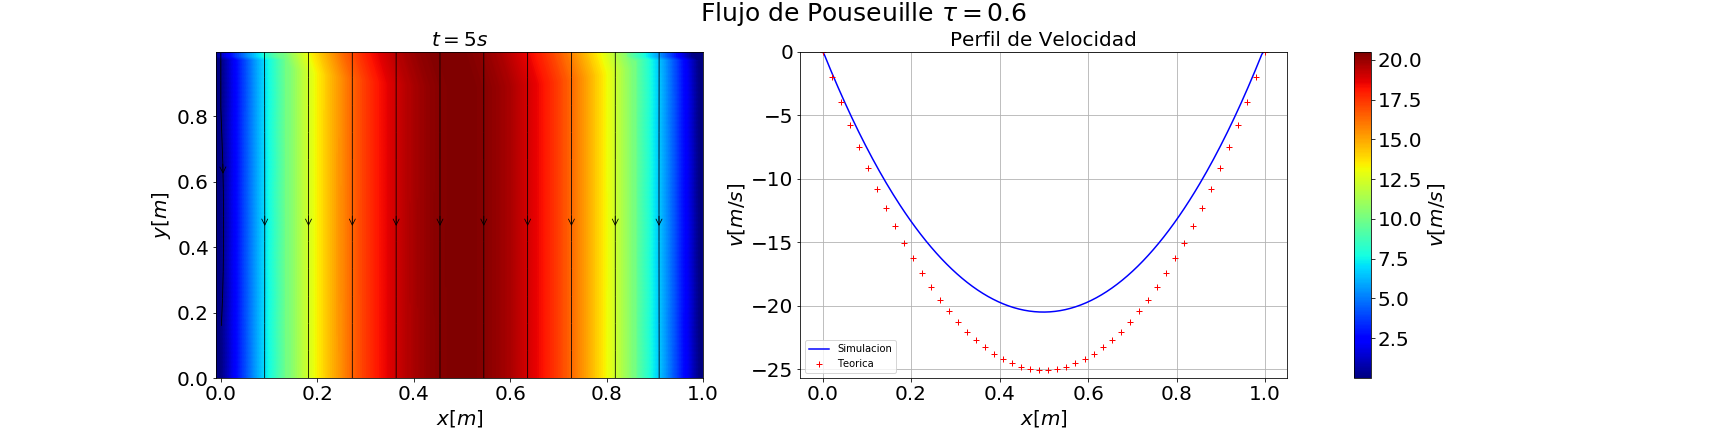
\includegraphics[scale=0.32]{5s.png} 
%\caption{Price regulation} \label{fig:timing3}
 \end{subfigure}
 
\begin{subfigure}
\centering
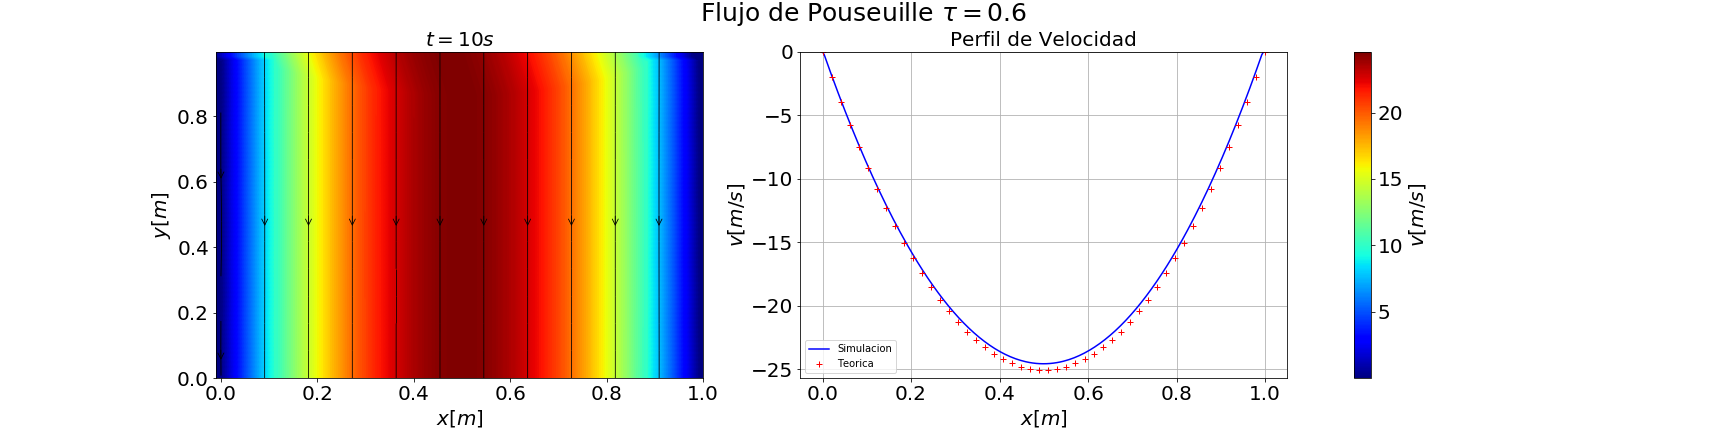
\includegraphics[scale=0.32]{10s.png} 
%\caption{Price regulation} \label{fig:timing3}
 \end{subfigure}

 \caption{Resultados simulación implementada en lattice Boltzmann para el flujo de Pouiseuille}


\end{figure}


\noindent para elegir las cantidades adecuadas al momento de representar las cantidades físicas reales , se ataca el problema de la siguiente manera. Denotando las unidades de lattice con el súper índice $^{*}$ . Dado que se conoce la solución teórica planteada en  \eqref{TeoricaPoiseuille} y teniendo en cuenta la ley de Poiseuille 

\begin{eqnarray}
u^{*} = \frac{g^{*}d^{*}}{8\nu^{*}}
\end{eqnarray}

\noindent se puede fijar $u^{*}=0.1$ para asegurar la stabilidad del código \cite{kruger}. Conocemos entonces el valor de la viscocidad en unidades de lattice y está dada de la siguiente manera

\begin{eqnarray}
\nu^{*} = (c_{o}^{*})^{2}\left(\tau^{*}-\frac{1}{2}\right)
\end{eqnarray}

\noindent entonces para encontrar el valor $\nu^{*}$ = 1/30, se elige $\tau =0.6$, esta elección determina las unidades correctas, para un sistema estable,  de la gravedad en unidades de lattice, obteniendose un valor del orden $g^{*} \approx 4\times 10^{-7}$. Además también se puede encontrar el número de Reynolds del sistema, encontrando

\begin{eqnarray}
Re = \frac{l^{*}u^{*}}{\nu^{*}} = \frac{lu}{\nu} =771
\end{eqnarray}

\noindent y desde acá se encuentra el paso de tiempo físico, dado por 

\begin{eqnarray}
\Delta t =(c_{o}^{*})^{2}\left(\tau^{*}-\frac{1}{2}\right)\frac{\Delta x^{2}}{\nu} =1.5\times 10^{-5}s
\end{eqnarray}

\noindent es decir que para que obtengamos el paso de tiempo de $t = 1s$, el sistema tiene que dar aproximadamente $66.000$ iteraciones. 

\medskip

\noindent para poder validar la simulación debemos comparar el resultado teórico y el resultado del perfil de velocidades obtenido en la simulación, esto se hace en la figura \ref{perfiles}, teniendo en cuenta que los factores de escala del sistema están dado por $dx = 1/256$ m, $1.5\times 10^{-5}$s. Esto asegura la validez del modelo planteado.


\subsection{Fluido en un cavidad}

Se presenta un flujo estacionario 2D en una cavidad cuadrada, utilizando el modelo lattice botlzmann con un lattice D2Q9. Este ejemplo es de mucha importancia dado que busca encontrar la validación del código a trevés de resultados conocidos. La configuración de este problema se muestra a continuación 


\begin{figure}[H]
\centering
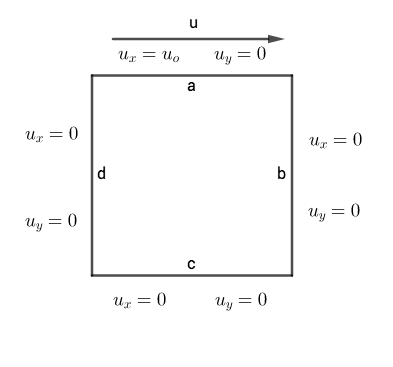
\includegraphics[scale = 0.6]{cavidad.png}
\caption{Esquema para el fluido en una cavidad}
\label{Poiseuille_100}
\end{figure}

\noindent El fluido está caracterizado por considerar un velocidad en el eje $x$ en la cara $a$, con magnitud $u_{o}$. El sistema está caracterizado por el número de Reynolds $Re = Lu_{o}/\nu$, donde $L$ es el lado del cuadrado ABCD y $\nu$ la viscosidad cinemática del fluido. Para las condiciones de frontera se utiliza el tradicional método bounce back \cite{kruger}. Para encontrar el número de Reynolds en la simulación se utiliza la expresión encontrada desde las ecuaciones de Navier Stokes partiendo del analisis de lattice Boltzmann

\begin{eqnarray}
Re = \frac{l u_{o}}{c_{o}^{2}(\tau - 0.5)}
\end{eqnarray}

\noindent En la simulación el tamaño del Lattice es de 256 x 256 y la velocidad de lado $a$ del cuadrado es $u_{o}= 0.1$, en donde el número de reynolds depende del tiempo de relajación. Los resultados obtenidos se presentan en las figuras siguientes

\begin{figure}[H]
\label{fig:Cavidad}
  \centering
  \begin{minipage}[b]{0.4\textwidth}
    \label{cavidadRe400}
    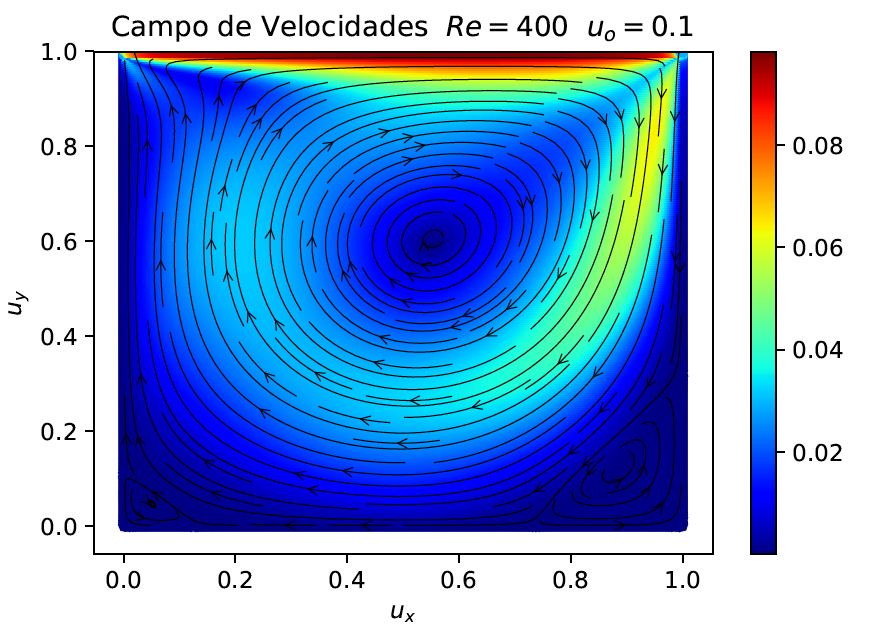
\includegraphics[scale =0.25]{cavidadRE400.png}
    %\caption{Fluido en una cavidad con un número de Reynolds de $Re = 400$}
  \end{minipage}
  \hspace{1cm}
  \begin{minipage}[b]{0.4\textwidth}
  \label{cavidadRe2000}
    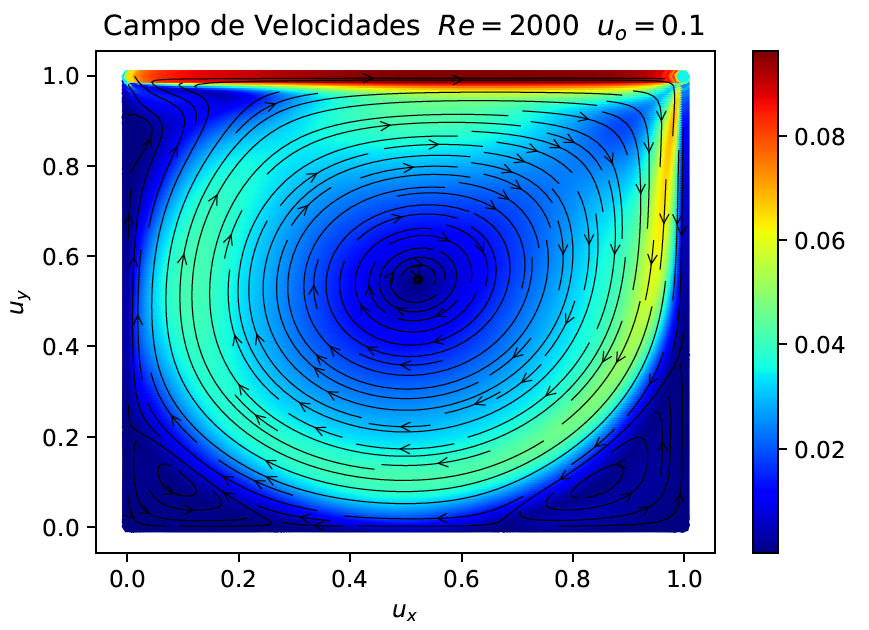
\includegraphics[scale=0.25]{cavidadRE200.png}
    %\caption{Fluido en una cavidad con un número de Reynolds de $Re = 2000$}
  \end{minipage}
  \caption{Fluido en una cavidad cuadrada con velocidad $u_{x} = 0.1$}
\end{figure}

Las lineas de corriente que se obtuvieron muestran claramente la formación de tres vórtices, uno principal en el centro del cuadrado y dos en las esquinas contrarias, es decir en el lado $c$. El efecto del número de Reynolds es claro al comparar los resultados en cuanto más grande sea tal número la tendencia a formar vórtices dentro del fluido es más grande\footnote{El código implementado se puede encontrar en el siguiente \href{https://github.com/jomen93/Cavidad_2D}{link}}.



